\documentclass[12pt]{article}
\hyphenpenalty=10000
\usepackage[swedish]{babel}
\usepackage{amsmath}
\usepackage{graphicx}

\title{Omfångsrikt problem: Mätning med märkning}
\author{Lukas Anderson}
\date{Maj 2023}

\begin{document}
\maketitle

\section{Problemförklaring}
Ett företag ska designa en serie nya skålar. En av skålarna ska ha en cirkulär bottenyta med radien 7 cm och en cirkulär öppning med radien 12 cm. Skålens höjd ska vara 13 cm och dess ytterkant sedd från sidan ska kunna approximeras med kurvan $y=kx^2-m$ som visas i Figur 1.

\begin{figure}[h]
    \centering
    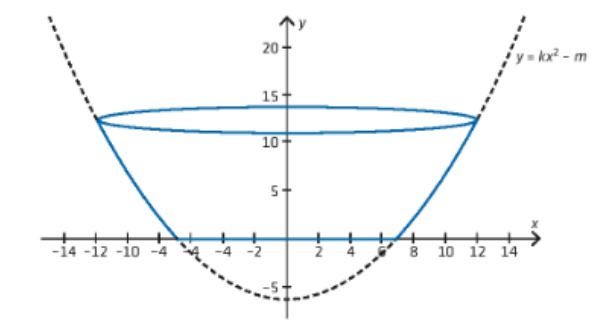
\includegraphics[width=\textwidth]{figur1.png}
    \caption{Skålens utseende}
\end{figure}

\subsection*{Uppgifter}
\begin{list}{-}{\leftmargin=1em\rightmargin=1em}
    \item Bestäm skålens volym med hjälp av {\it skivmetoden}.
    \item Designa två liknande skålar vars respektive volym är 3 liter.
    \item Eftersom skålarna är tänkta att användas vid bakning, så vill företaget att man på insidan av skålen ska kunna läsa av volymen. En av dina treliters-skålar ska ha sådana märkningar för varje liter. Bestäm på vilka höjder dessa märkningar ska sitta.
    \item Ta reda på hur man använder integraler för att beräkna volym med hjälp av {\it skalmetoden}.Redogör för hur metoden fungerar och lista ut hur du kan använda den för att beräkna volymen av någon av skålarna ovan. Beräkna också den volymen.
    \item Du behärskar nu två olika metoder för att beräkna volymen av en rotationskropp: {\it skivmetoden\/} och {\it skalmetoden}. Diskutera metodernas för- och nackdelar.
\end{list}

\section{Uppgift 1}
\subsection*{Bestäm skålens volym med hjälp av {\it skivmetoden}.}

Formeln för skivmetoden är $V=\pi\int_{0}^{13}{g(y)}^2dy$
Där funktionen $g(y)$ är $f(x)$ uttryckt som en funktion av $y$.
\\\\
För att finna $g(y)$ identifierar vi först funktionen $f(x)=y$ som beskriver skålens form och kan beskrivas som $y=kx^2-m$. Att skålen har radien 7 cm innebär att $f(x)$ har rötterna $(7,0) (-7,0)$
För att finna $k$ och $m$ löser ställer vi upp följande ekvation:\\
\begin{align*}
    kx^2-m&=k(x-7)(x+7)\\
    kx^2-m&=k(x^2-49)\\
    kx^2-m&=kx^2-49k\\
    m&=49k\\
\end{align*}
Vilket ger oss att $m=49k$ och att $f(x)=y=kx^2-49k$.
\\\\
För att finna $k$ löser vi följande ekvation:
\begin{align*}
    f(12)=13\\
    13&=k{(12)}^2-49k\\
    13&=144k-49k\\
    13&=95k\\
    k&=\frac{13}{95}\\
\end{align*}
Vilket ger oss att $k=\frac{13}{95}$ och att $f(x)=y=\frac{13}{95}x^2-\frac{637}{95}$.
\\\\
Detta visas i Figur 2.

\begin{figure}[h]
    \centering
    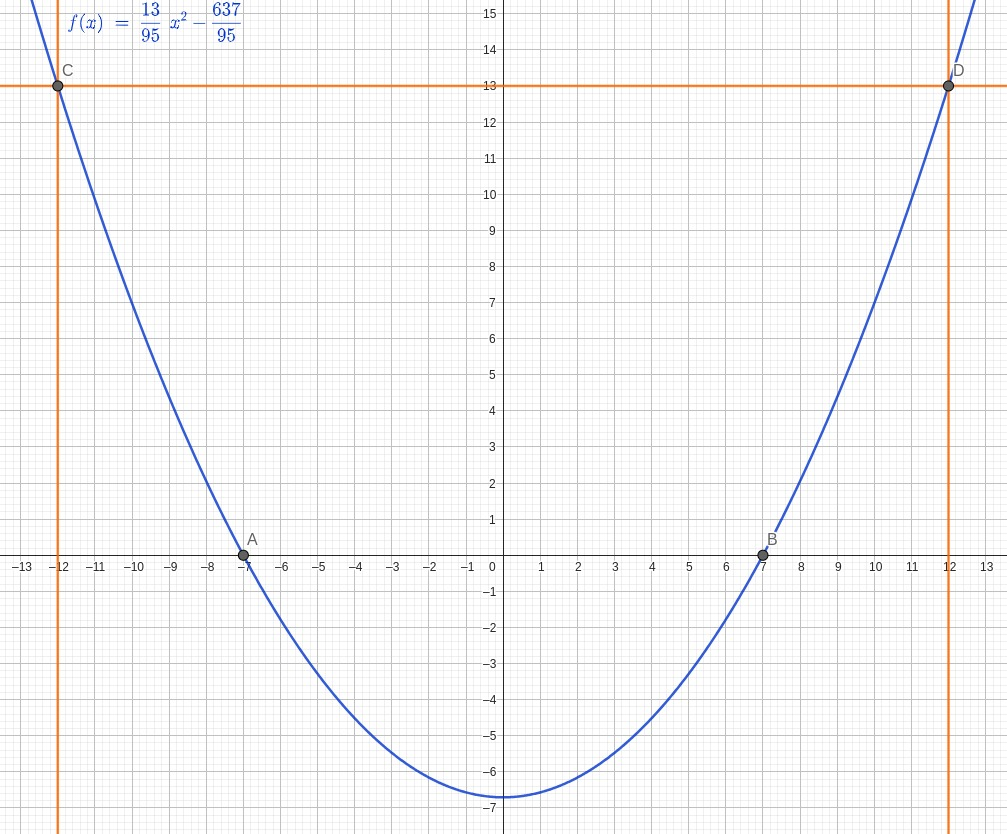
\includegraphics[width=0.8\textwidth]{figur2.jpg}
    \caption{Skålens utseende med $f(x)$ uttryckt som en funktion}
\end{figure}

\newpage
Med $f(x)=\frac{13}{95}x^2-\frac{637}{95}$ kan vi räkna ut $g{(y)}^2$ då $g(y)=x$ och $f(x)=y$:
\begin{align*}
    \frac{13}{95}x^2-\frac{637}{95}&=y\\
    \frac{13}{95}x^2&=y+\frac{637}{95}\\
    x^2&=\frac{y+\frac{637}{95}}{\frac{13}{95}}\\
    g{(y)}^2&=\frac{y+\frac{637}{95}}{\frac{13}{95}}\\
    g{(y)}^2&=\frac{95y+637}{13}\\
\end{align*}
Detta ger oss att $g{(y)}^2=\frac{95y+637}{13}$.
För att räkna ut volymen med formeln $V=\pi\int_{0}^{13}{g(y)}^2dy$ måste vi först bestämma den primitiva funktionen $H(y)$ till funktionen $h(y)=g{(y)}^2=\frac{95y+637}{13}$.

\begin{align*}
    h(y)&=\frac{95y+637}{13}\\
    h(y)&=\frac{95}{13}y+\frac{637}{13} \Rightarrow H(y)=\frac{95/13}{2}y^2+\frac{637}{13}y+C\\
    H(y)&=\frac{95}{26}y^2+\frac{637}{13}y+C\\
\end{align*}
Detta ger oss att $H(y)=\frac{95}{26}y^2+\frac{637}{13}y+C$.
\newpage
Vi kan nu skriva om formeln $V=\pi\int_{0}^{13}{g(y)}^2dy$:
\begin{align*}
    V&=\pi\int_{0}^{13}{g(y)}^2dy\\
    V&=\pi\int_{0}^{13}{h(y)}dy\\
    V&=\pi\int_{0}^{13}{h(y)}dy\Rightarrow V=\pi{\left[{H(y)}\right]}_{0}^{13}\\
    V=\pi{\left[{H(y)}\right]}_{0}^{13}&=\pi\left(\frac{95}{26}{(13)}^2+\frac{637}{13}(13)-\frac{95}{26}{(0)}^2-\frac{637}{13}(0)\right)\\
    V&=\pi\left(\frac{95}{26}{(13)}^2+\frac{637}{13}(13)\right)\\
    V&=\pi\left(\frac{95}{26}{(169)}+\frac{637}{13}(13)\right)\\
    V&=\pi\left(\frac{16055}{26}+\frac{8271}{13}\right)\\
    V&=\frac{16055\pi}{26}+\frac{8271\pi}{13}\\
    V&\approx 3938.7\text{ cm}^3\\
\end{align*}
skivmetoden get oss att skålen har volymen $V\approx 3938.7\text{ cm}^3$.
\newpage
\section{Uppgift 2}
\subsection*{Designa två liknande skålar vars respektive volym är 3 liter.}

För att designa två liknande skålar vars respektive volym är 3 liter börjar med att bestämma radien av skålens bottenyta. För den första skålen Skål 1, bestämmer jag att radien ska vara 4 cm. För den andra skålen Skål 2, bestämmer jag att radiens ska vara 6 cm.
\\\\
\subsection*{Skål 1:}
För att bestämma skålens form börjar jag med att bestämma funktionen $f(x)$ som beskriver skålens form. Jag bestämmer att skålen ska ha en bottenyta med radien 4 cm. Detta innebär att $f(x)$ har rötterna $(4,0) (-4,0)$ och att $f(x)=k(x-4)(x+4)$. $k$ i funktionen bestämmer hur aggresiv lutningen är på skålens sidor. Jag bestämmer att $k=0.1$ vilket ger mig att \\ $f(x)=0.1(x-4)(x+4)$.
\\\\
Funktionen $f(x)$ kan då skrivas i formen $kx^2-m$:

\begin{align*}
    f(x)&=0.1(x-4)(x+4)\\
    f(x)&=0.1(x^2-16)\\
    f(x)&=0.1x^2-1.6\\
\end{align*}




\end{document}